\scanpage{84}
% @0 upper right
\mspage{- 22 -}
% @1–2 proposition
\noindent\begin{tikzpicture}
\node[inner sep=3pt] (prop) {\begin{minipage}{.89\linewidth}
\uline{Proposition 3.1} : Soient $C$ un site annelé et $\unsure{G|C}$ un faisceau d\handwritten{e} $A$-modules sur $C$. Les conditions suivantes sont équivalentes :

% @3–4 condition i
i) Pour tout objet $X$ de $C$ et tout crible couvrant $R\handwritten{\hookrightarrow}X$
\[
 H^q(C^{\wedge}/R,\handwritten{\mathscr H}^0(G))=0\qquad\handwritten{\forall}\ q\handwritten{>}0
\]
% @5–6 condition ii
ii) Pour tout objet $X$ de $C$
\[
 \handwritten{\check}{H}^q(C^{\wedge}/X,\handwritten{\mathscr H}^0(G))=0\qquad\handwritten{\forall}\ q\handwritten{>}0
\]
% @7 ii bis
ii)$^{\mathrm{bis}}$ Les préfaisceaux $\handwritten{\check{\mathscr H}}^q\,\handwritten{\mathscr H}^0(G)$ sont nuls pour tout $q\handwritten{>}0$.

% @8–9 condition iii
iii) Pour tout objet $X$ de $C$
\[
 H^q(C^{\handwritten{\sim}}/X,G)=0\qquad\handwritten{\forall}\ q\handwritten{>}0
\]
% @10 iii bis
iii)$^{\mathrm{bis}}$ Les préfaisceaux $\handwritten{\mathscr H}^q(G)$ sont nuls pour tout $q\handwritten{>}0$.
\end{minipage}};
\handwritten{\draw (prop.north west) ++(2pt,1pt) -- (prop.north west) -- (prop.south west) -- ++(2pt,-1pt);}
\end{tikzpicture}

% @11–17 proof
\uline{Preuve} : Il est clair qu'on a les équivalences $(\mathrm{ii})\handwritten{\Longleftrightarrow}(\mathrm{ii})^{\mathrm{bis}}$ (N$^\circ$ 2, formules (14) et (15)) et $(\mathrm{iii})\handwritten{\Longleftrightarrow}(\mathrm{iii})^{\mathrm{bis}}$ (N$^\circ$ 2, formule (12)). D'autre part, on a l'implication $(\mathrm{i})\handwritten{\Longrightarrow}(\mathrm{ii})$ \handwritten{(}N$^\circ$ 2, formule (14)) et l'implication $(\mathrm{iii})^{\mathrm{bis}}\handwritten{\Longrightarrow}(\mathrm{i})$ par la suite spectrale de la proposition 2.3 Il nous reste donc à montrer l'implication $(\mathrm{ii})^{\mathrm{bis}}\handwritten{\Longrightarrow}(\mathrm{iii})^{\mathrm{bis}}$ qui résulte immédiatement de la dernière assertion de (2.5) c.q.f.d.

% @18–20 definition
\noindent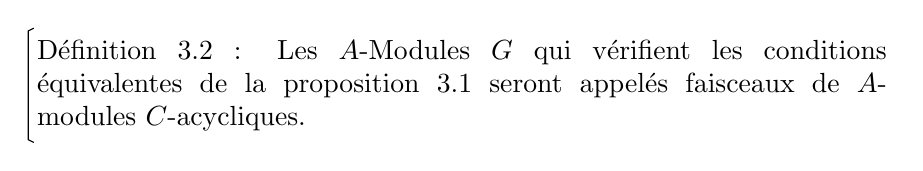
\begin{tikzpicture}
\node[inner sep=3pt] (defn) {\begin{minipage}{.89\linewidth}
\uline{Définition 3.2} : Les $A$-Modules $G$ qui vérifient les conditions équivalentes de la proposition 3.1 seront appelés faisceaux de $A$-modules \uline{$C$-acycliques}.
\end{minipage}};
\handwritten{\draw (defn.north west) ++(2pt,1pt) -- (defn.north west) -- (defn.south west) -- ++(2pt,-1pt);}
\end{tikzpicture}
% @21 foot
\hfill \ldots/\ldots
% archive sheet number: 83

